\documentclass{article}

% Packages in popl2018.tex
%\usepackage{latexsym}
%\usepackage{setspace}
%\usepackage{cancel}
%\usepackage{listings}
%\usepackage{graphicx}
%\usepackage{appendix}
%\usepackage{amssymb}
%\usepackage{stmaryrd}
%\usepackage{amsmath}
%\usepackage{leftidx}
\usepackage{mathtools}
%\usepackage{paralist}
\usepackage{color}
%\usepackage{mathrsfs}
\usepackage{tikz}
%\usetikzlibrary{shapes}
%\usepackage[linesnumbered,ruled]{algorithm2e}


% New packages
\usetikzlibrary{automata,positioning}

\newtheorem{theorem}{Theorem}
\newtheorem{definition}{Definition}

%==========================================================

% General
\newcommand\brac[1]{\left(#1\right)}
\newcommand\tup\brac


% Tiling

\newcommand\width{\ell}
\newcommand\height{h}
\newcommand\hcons{H}
\newcommand\vcons{V}
\newcommand\tiles{T}
\newcommand\tile{t}
\newcommand\inittile{t_0}
\newcommand\fintile{t_f}
\newcommand\rowdelim{\#}

% Reduction
\newcommand\resetchar{!}
\newcommand\bit{b}

% \nbit[i][0] = 0_i, similarly for 1
\newcommand\nbit[2]{#2_{#1}}

% \repl{n}{0}{1} = $^1_{n,0} means if nth bit is 0, turn into a 1
\newcommand\repl[3]{\$^{#3}_{#1, #2}}

%!TEX root = popl2018.tex

\newcommand{\set}[1]{\{ #1 \}}
\newcommand{\sequence}[2]{(#1, \ldots, #2)}
\newcommand{\couple}[2]{(#1,#2)}
\newcommand{\pair}[2]{(#1,#2)}
\newcommand{\triple}[3]{(#1,#2,#3)}
\newcommand{\quadruple}[4]{(#1,#2,#3,#4)}
\newcommand{\tuple}[2]{(#1,\ldots,#2)}
\newcommand{\Nat}{\ensuremath{\mathbb{N}}}
\newcommand{\Rat}{\ensuremath{\mathbb{Q}}}
\newcommand{\Rea}{\ensuremath{\mathbb{R}}}
\newcommand{\Zed}{\ensuremath{\mathbb{Z}}}
%\newcommand{\true}{\top}
%\newcommand{\false}{\perp}
\newcommand{\bottom}{\perp}
%% \newcommand{\powerset}[1]{{\cal P}(#1)}
\newcommand{\npowerset}[2]{{\cal P}^{#1}(#2)}
\newcommand{\finitepowerset}[1]{{\cal P}_f(#1)}
\newcommand{\level}[2]{L_{#1}(#2)}
\newcommand{\card}[1]{\mbox{card}(#1)}
\newcommand{\range}[1]{\mathtt{ran}(#1)}
\newcommand{\astring}{s}

\newcommand{\Cc}{\mathcal{C}}


\newcommand {\notof}{\ensuremath{\neg}}
\newcommand {\myand}{\ensuremath{\wedge}}
\newcommand {\myor}{\ensuremath{\vee}}
\newcommand {\mynext}{\mbox{{\sf X}}}
\newcommand {\until}{\mbox{{\sf U}}}
\newcommand {\sometimes}{\mbox{{\sf F}}}
\newcommand {\previous}{\mynext^{-1}}
\newcommand {\since}{\mbox{{\sf S}}}
\newcommand {\fminusone}{\mbox{{\sf F}}^{-1}}
\newcommand {\everywhere}[1]{\mbox{{\sf Everywhere}}(#1)}



\newcommand{\aatomic}{{\rm A}}
\newcommand{\aset}{X}
\newcommand{\asetbis}{Y}
\newcommand{\asetter}{Z}

\newcommand{\avarprop}{p}
\newcommand{\avarpropbis}{q}
\newcommand{\avarpropter}{r}
\newcommand{\varprop}{{\rm PROP}} % Set of atomic propositions (for a given logic)

% formulae

\newcommand{\aformula}{\astateformula} % a formula
\newcommand{\aformulabis}{\astateformulabis} % another formula (when at least 2 are present)
\newcommand{\aformulater}{\astateformulater} % another formula (when at least 3 are present)
\newcommand{\asetformulae}{X}
\newcommand{\subf}[1]{sub(#1)}

\newcommand{\aautomaton}{{\mathbb A}}
\newcommand{\aautomatonbis}{{\mathbb B}}

\newcommand {\length}[1] {\ensuremath{|#1|}}



% Equivalences
\newcommand{\egdef}{\stackrel{\mbox{\begin{tiny}def\end{tiny}}}{=}} % =def=
\newcommand{\eqdef}{\stackrel{\mbox{\begin{tiny}def\end{tiny}}}{=}} % =def=
\newcommand{\equivdef}{\stackrel{\mbox{\begin{tiny}def\end{tiny}}}{\equivaut}} % <=def=>
\newcommand{\equivaut}{\;\Leftrightarrow\;}

\newcommand{\ainfword}{\sigma}

\newcommand{\amap}{\mathfrak{f}}
\newcommand{\amapbis}{\mathfrak{g}}

\newcommand{\step}[1]{\xrightarrow{\!\!#1\!\!}}
\newcommand{\backstep}[1]{\xleftarrow{\!\!#1\!\!}}

\newcommand {\aedge}[1] {\ensuremath{\stackrel{#1}{\longrightarrow}}}
\newcommand {\aedgeprime}[1] {\ensuremath{\stackrel{#1}{\longrightarrow'}}}
\newcommand {\afrac}[1] {\ensuremath{\mathit{frac}(#1)}}
\newcommand {\cl}[1] {\ensuremath{\mathit{cl}(#1)}}
\newcommand {\sfc}[1] {\ensuremath{\mathit{sfc}(#1)}}
\newcommand {\dunion} {\ensuremath{\uplus}}
\newcommand {\edge} {\ensuremath{\longrightarrow}}
\newcommand {\emptyword}{\ensuremath{\epsilon}}
\newcommand {\floor}[1] {\ensuremath{\lfloor #1 \rfloor}}
\newcommand {\intersection} {\ensuremath{\cap}}
\newcommand {\union} {\ensuremath{\cup}}
\newcommand {\vals}[2] {\ensuremath{\mathit{val}_{#2}(#1)}}



\newcommand {\pspace} {\textsc{pspace}}
\newcommand {\nlogspace} {\textsc{nlogspace}}
\newcommand {\logspace} {\textsc{logspace}}
\newcommand {\expspace} {\textsc{expspace}}
\newcommand {\np} {\textsc{np}}
\newcommand {\threeexptime} {\textsc{3exptime}}
\newcommand {\polytime} {\textsc{p}}
\newcommand{\twoexpspace}{\textsc{2expspace}}
\newcommand{\threeexpspace}{\textsc{3expspace}}
\newcommand {\nexptime} {\textsc{nexptime}}



\newcommand{\aalphabet}{\Sigma}     % an alphabet, A is already used for atoms
\newcommand{\aword}{\mathfrak{u}}
\newcommand{\awordbis}{\mathfrak{v}}



\newcommand{\aassertion}{P}
\newcommand{\aassertionbis}{Q}
\newcommand{\aexpression}{e}
\newcommand{\aexpressionbis}{f}
\newcommand{\avariable}{\mathtt{x}}
\newcommand{\uniquevar}{\mathtt{u}}
\newcommand{\uniquevarbis}{\mathtt{v}}
\newcommand{\avariablebis}{\mathtt{y}}
\newcommand{\avariableter}{\mathtt{z}}
\newcommand{\nullconstant}{\mathtt{null}}
\newcommand{\nilvalue}{nil}
\newcommand{\emptyconstant}{\mathtt{emp}}
\newcommand{\infheap}{\mathtt{inf}}
\newcommand{\saturated}{\mathtt{Saturated}}

\newcommand{\astateformula}{\phi}
\newcommand{\astateformulabis}{\psi}
\newcommand{\astateformulater}{\varphi}
%%
\newcommand{\separate}{\ast}
\newcommand{\sep}{\separate}
\newcommand{\size}{\mathtt{size}}
\newcommand{\sizeeq}[1]{\mathtt{size} \ = \ #1}
\newcommand{\alloc}[1]{\mathtt{alloc}(#1)}
\newcommand{\allocb}[2]{\mathtt{alloc}^{-1}[#2](#1)}
\newcommand{\isol}[1]{\mathtt{isoloc}(#1)}
\newcommand{\icell}{\mathtt{isocell}}
\newcommand{\malloc}{\mathtt{malloc}}
\newcommand{\cons}{\mathtt{cons}}
\newcommand{\new}{\mathtt{new}}
\newcommand{\free}[1]{\mathtt{free} \ #1}
\newcommand{\maxform}[1]{\mathtt{maxForms}(#1)}
\newcommand{\locations}[1]{\mathtt{loc}(#1)}
\newcommand{\values}{\mathtt{Val}}
\newcommand{\aheap}{\mathfrak{h}}
\newcommand{\avaluation}{\mathfrak{V}}
\newcommand{\heaps}{\mathcal{H}}
\newcommand{\astore}{\mathfrak{s}}
\newcommand{\stores}{\mathcal{S}}
\newcommand{\amodel}{\mathfrak{M}}
\newcommand{\alabel}{\ell}

\newcommand{\aprogram}{\mathtt{PROG}}
\newcommand{\programs}{\mathtt{P}}
\newcommand{\ctprograms}{\programs^{ct}}
\newcommand{\aninstruction}{\mathtt{instr}}
\newcommand{\ainstruction}{\mathtt{instr}}
\newcommand{\instructions}{\mathtt{I}}
\newcommand{\aguard}{\ensuremath{g}}
\newcommand{\guards}{\ensuremath{G}}
\newcommand{\domain}[1]{\mathtt{dom}(#1)}
\newcommand{\memory}{\stores\times\heaps}
\newcommand{\skipinstruction}{\mathtt{skip}}

\newcommand{\execution}{\mathtt{comp}}
\newcommand{\aux}{\mathtt{embd}}
\newcommand{\runof}{run}
\newcommand{\anexecution}{e}


\newcommand{\aletter}{\ensuremath{a}}
\newcommand{\aletterbis}{\ensuremath{b}}
\newcommand{\alocation}{\mathfrak{l}}

\newcommand{\pointsl}[1]{\stackrel{#1}{\hookrightarrow}}
\newcommand{\ppointsl}[1]{\stackrel{#1}{\mapsto}}
\newcommand{\ourhook}[1]{\stackrel{#1}{\hookrightarrow}}
\newcommand{\ltrue}{{\sf true}}
\newcommand{\lfalse}{{\sf false}}


\newcommand{\variables}{\mathtt{FVAR}}
\newcommand{\pvariables}{\mathtt{PVAR}}
\newcommand{\secvariables}{\mathtt{SVAR}}
\newcommand{\logique}[1]{\mathtt{FO}(#1)}



\newcommand{\atranslation}{\mathfrak{t}}
\newcommand{\nbpred}[1]{\widetilde{\sharp #1}}
\newcommand{\nbpredstar}[1]{\widetilde{\sharp #1}^{\star}}
\newcommand{\isolated}{\mathtt{isol}}
\newcommand{\stdmarks}{\mathtt{envir}}
\newcommand{\relation}[1]{\mathtt{relation}_{#1}}
\newcommand{\freevar}{\mathtt{FV}}
\newcommand{\notonmark}{\mathtt{notonenv}}
\newcommand{\InVal}[1]{\mathtt{InVal}\!\left(#1\right)}
\newcommand{\NotOnEnv}[1]{\mathtt{NotOnEnv}\!\left(#1\right)}
\newcommand{\PartOfVal}[1]{\mathtt{PartOfVal}\!\left(#1\right)}
%\newcommand{\nbpreds}[3]{\sharp #1 \geq #2}
\newcommand{\defstyle}[1]{{\emph{#1}}}

\newcommand{\cut}[1]{}
\newcommand{\interval}[2]{[#1,#2]}
\newcommand{\buniquevar}{\overline{\uniquevar}}
\newcommand{\bbuniquevar}{\overline{\overline{\uniquevar}}}
\newcommand{\magicwand}{\mathop{\mbox{$\mbox{$-~$}\!\!\!\!\ast$}}}
\newcommand{\wand}{\magicwand}
\newcommand{\septraction}{\stackrel{\hsize0pt \vbox to0pt{\vss\hbox to0pt{\hss\raisebox{-6pt}{\footnotesize$\lnot$}\hss}\vss}}{\magicwand}}
%% \newcommand{\reach}{\mathtt{reach}}
\mathchardef\mhyphen="2D % hyphen while in math mode

\newcommand{\adataword}{\mathfrak{dw}}
\newcommand{\adatum}{\mathfrak{d}}

\newcommand{\collectionknives}{\mathtt{ks}}
\newcommand{\collectionknivesfork}[1]{\mathtt{ksfs}_{=#1}}
\newcommand{\collectionknivesforks}{\mathtt{ksfs}}
\newcommand{\collectionkniveslargeforks}{\mathtt{kslfs}}


\newcommand{\acounter}{\mathtt{C}}

\newcommand{\fotwo}[3]{{\mbox{FO2}_{#1,#2}(#3)}}
\newcommand{\mtrans}[1]{t\!\left(#1\right)^{\Box}}
\newcommand{\mbtrans}[2]{\mtrans{#2}_{#1}}


\newcommand{\alogic}{\mathfrak{L}}


\newcommand{\semantics}[1]{\ensuremath{[ #1 ]}}


\newcommand{\adomino}{\mathfrak{d}}
\newcommand{\atile}{\mathfrak{d}}
\newcommand{\atiling}{\mathfrak{t}}

\newcommand{\hori}{\mathtt{h}}
\newcommand{\verti}{\mathtt{v}}
\newcommand{\domi}{\mathtt{d}}

\newcommand{\cpyrel}{\mathfrak{cp}}

\newcommand{\cntcmp}{\mathfrak{C}}

\newcommand{\heapdag}{\mathfrak{G}}

\newcommand{\onmainpath}{\mathtt{mp}}

\newcommand{\tree}{\mathtt{tree}}

%\newcommand{\tile}{\mathtt{tile}}

\newcommand{\type}{\mathtt{type}}

\newcommand{\ptype}{\mathtt{ptype}}

\newcommand{\exttype}{\mathtt{exttype}}

\newcommand{\anctypes}{\mathtt{AncTypes}}

\newcommand{\destypes}{\mathtt{DesTypes}}

\newcommand{\inctypes}{\mathtt{IncTypes}}

\newcommand{\treeic}{\mathtt{treeIC}}

\newcommand{\trs}{\mathfrak{trs}}


\newcommand{\nin}{\not \in}
\newcommand{\cupplus}{\uplus}
\newcommand{\aunarypred}{\mathtt{P}}


\newcommand{\hide}[1]{}

\newcommand{\eval}[2]{\llbracket#1\rrbracket_{#2}}
\newcommand\cur{\mathsf{cur}}
\newcommand\dom{\mathsf{dom}}
\newcommand\rng{\mathsf{rng}}

\newcommand\dd{\mathbb{D}}
\newcommand\nat{\mathbb{N}}


\newcommand\cA{\mathcal{A}}
\newcommand\cB{\mathcal{B}}
\newcommand\cC{\mathcal{C}}
\newcommand\cE{\mathcal{E}}
\newcommand\cG{\mathcal{G}}
\newcommand\Ll{\mathcal{L}}
\newcommand\cM{\mathcal{M}}
\newcommand\cP{\mathcal{P}}
\newcommand\cR{\mathcal{R}}
\newcommand\cS{\mathcal{S}}
\newcommand\cT{\mathcal{T}}

\newcommand\vard{\mathfrak{d}}

\newcommand\replaceall{\mathsf{replaceAll}}
\newcommand\indexof{\mathsf{IndexOf}}


\newcommand\strline{\mathsf{SL}}

\newcommand\pstrline{\mathsf{SL_{pure}}}

\newcommand\search{\mathsf{search}}

\newcommand\verify{\mathsf{verify}}

\newcommand\searchleft{\mathsf{searchLeft}}

\newcommand\searchlong{\mathsf{searchLong}}


\newcommand\pref{\mathsf{Pref}}

\newcommand\wprof{\mathsf{WP}}

\newcommand\vars{\mathsf{Vars}}

\newcommand\dep{\mathsf{Dep}}
\newcommand\ptn{\mathsf{Ptn}}

\newcommand\src{\mathsf{src}}
\newcommand\strtorep{\mathsf{strToRep}}

\newcommand\rpleft{\mathsf{l}}
\newcommand\rpright{\mathsf{r}}


\newcommand\srcnd{\mathsf{srcND}}

\newcommand\ctxt{\mathsf{ctxt}}


\newcommand\ctxts{\mathsf{Ctxts}}

\newcommand\sprt{\mathsf{sprt}}

\newcommand\val{\mathsf{val}}

\newcommand\srclen{\mathsf{srcLen}}

\newcommand\rpleftlen{\mathsf{lLen}}


\newcommand\dfs{\mathsf{DFS}}

\newcommand\repr{\mathsf{rep}}

\newcommand\red{\mathsf{red}}

\newcommand\gfun{\mathcal{F}}


\newcommand{\leftmost}{{\sf leftmost}}
\newcommand{\longest}{{\sf longest}}

\newcommand{\arbidx}{{\sf Idx_{arb}}}
\newcommand{\dmdidx}{{\sf Idx_{dmd}}}
\newcommand{\lftlen}{{\sf Len_{lft}}}

%\newtheorem{remark}[theorem]{Remark}

\newcommand{\OMIT}[1]{}
\newcommand{\defn}[1]{\emph{#1}}

\newcommand{\Left}{\ensuremath{-1}}
\newcommand{\Right}{\ensuremath{1}}
\newcommand{\Stay}{\ensuremath{0}}

\newcommand{\Aut}{\ensuremath{\mathcal{A}}}
\newcommand{\AutB}{\ensuremath{\mathcal{B}}}
\newcommand{\Transducer}{\ensuremath{T}}
\newcommand{\controls}{\ensuremath{Q}}
\newcommand{\finals}{\ensuremath{F}}
\newcommand{\transrel}{\ensuremath{\delta}}

\newcommand{\Lang}{\mathcal{L}}
\newcommand{\Tran}{\mathcal{T}}

\newcommand{\ialphabet}{\Sigma}
\newcommand{\oalphabet}{\Gamma}

\newcommand{\EndLeft}{\ensuremath{\vartriangleright}}
\newcommand{\EndRight}{\ensuremath{\vartriangleleft}}



%==========================================================

\newcommand{\anthony}[1]{\color{red} {YA: #1 :AY} \color{black}}
\newcommand{\zhilin}[1]{\color{brown} {ZL: #1 :LZ} \color{black}}
\newcommand{\tl}[1]{\color{blue} {TL: #1 :LT} \color{black}}
\newcommand{\mat}[1]{\color{cyan} {MH: #1 :HM} \color{black}}

\newcommand{\concat} {\circ}
\newcommand{\replace} {{\sf replace}}
\newcommand{\str} {{\sf Str}}
\newcommand{\intnum} {{\sf Int}}
\newcommand{\regexp} {{\sf RegExp}}
\newcommand{\strarr} {{\sf StringArray}}
\newcommand{\dtypes} {{\sf DataTypes}}
\newcommand{\anarr} {{\mathbb{A}}}

%============================================================


\title{EXPSPACE-hardness of $\strline[\replaceall]$}
\author{Taolue Chen, Matthew Hague, Anthony Widjaja Lin, Zhilin Wu \\ and Zhilin's Student (apologies, i have lost the name)}
\date{}

\begin{document}

\maketitle

We will attempt to show the following result.

\begin{theorem}
    Satisfiability of $\strline[\replaceall]$, even in the single-letter case, is EXPSPACE-hard.
\end{theorem}

To show the above result, we will give a constraint that represents a straight-line program which ``transforms'' an automaton into exponentially many different automata.
These exponentially many automata will be used to check the vertical tiling relation for a tiling problem with an exponentially wide corridor.
Since such tiling problems are EXPSPACE-hard, the result follows.

After introducing the tiling problem, we will show the form of the constraint without specifying the regular languages used.
We will then describe the effect that eliminating the $\replaceall$ and string concatenations has on the regular languages.
Then, we will give a simple example of how this effect may be used to generate interesting languages.
Finally, we will give the precise languages needed to obtain our result.

\section{Tiling Problems}

\begin{definition}[Tiling Problems]
    A \emph{tiling problem} is a tuple
    $\tup{\tiles, \inittile, \fintile, \hcons, \vcons, \width}$
    where
        $\tiles$ is a finite set of tiles,
        $\inittile, \fintile \in \tiles$ are initial and final tiles respectively,
        $\hcons, \vcons \in \tiles \times \tiles$
            are horizontal and vertical matching relations respectively, and
        $\width$ is the width of the tiling corridor.
\end{definition}

A solution to a tiling problem
$\tup{\tiles, \inittile, \fintile, \hcons, \vcons, \width}$
is a string
\[
    \rowdelim \tile^1_1 \cdots \tile^1_\width
    \rowdelim \tile^2_1 \cdots \tile^2_\width
    \rowdelim \cdots
    \rowdelim \tile^\height_1 \cdots \tile^\height_\width
    \rowdelim
\]
where $\rowdelim \notin \tiles$ is a delimiter, $\height$ is some positive integer, and
\begin{enumerate}
\item
    $\tile^1_1 = \inittile$,
\item
    $\tile^\height_\width = \fintile$,
\item
    $\tup{\tile^i_j, \tile^i_{j+1}} \in \hcons$
    for all
    $i \in [\height]$
    and
    $j \in [\width - 1]$, and
\item
    $\tup{\tile^i_j, \tile^{i+1}_j} \in \vcons$
    for all
    $i \in [\height - 1]$
    and
    $j \in [\width]$.
\end{enumerate}

The problem of determining whether a tiling problem has a solution is $\width$-SPACE-hard~\cite{TODO}.
\mat{TODO: add citation}


\section{Reduction}

Fix a tiling problem
$\tup{\tiles, \inittile, \fintile, \hcons, \vcons, \width}$
such that
$\width = 2^n$
for some $n$.
We will create a single-letter satisfiability problem of $\strline[\replaceall]$ which has a solution iff the tiling problem has a solution.

In particular, we will require that a certain variable $x_1$ can take a value
\[
    \resetchar
    \rowdelim \nbit{1}{0} \cdots \nbit{n}{0} \tile^1_1
              \nbit{1}{0} \cdots \nbit{n}{1} \tile^1_2
              \cdots
              \nbit{1}{1} \cdots \nbit{n}{1} \tile^1_\width
    \rowdelim \cdots
    \rowdelim \nbit{1}{0} \cdots \nbit{n}{0} \tile^\height_1
              \cdots
              \nbit{1}{1} \cdots \nbit{n}{1} \tile^\height_\width
    \rowdelim
    \resetchar
\]
where
$\resetchar,
 \nbit{1}{0}, \nbit{1}{1},
 \ldots,
 \nbit{n}{0}, \nbit{n}{1} \notin \tiles$.
In particular, the solution is a solution to the tiling problem, except each tile is preceded by a binary number of length $n$ encoding the number of the column in which it appears.
Note, we have a different character for each bit position, e.g. $\nbit{2}{0}$ is a distinct character from $\nbit{3}{0}$.
The $\resetchar$ will be used to mark the beginning and end of the word and is required for technical reasons.

To reach such a solution, we will use the constraints to effectively generate an exponential number of languages.
We can number these languages in binary, i.e.\ $L_{0\cdots00}$ to $L_{1\cdots11}$.
In addition to $\resetchar$, $\nbit{i}{0}$, and $\nbit{i}{1}$, we will also introduce characters of the form
$\repl{i}{\bit}{\bit'}$.
In language
$L_{\bit_1\cdots\bit_n}$,
the character
$\repl{i}{\bit}{\bit'}$
will mean that if $\bit_i = \bit$, then match the character
$\bit' \in \set{\nbit{i}{0},\nbit{i}{1}}$.
This will become clearer when we show an example, but first we will give the constraint needed to generate the languages.

\subsection*{The Constraint}

The constraint we will need to encode solutions to the tiling problem is below.
It gives a straight-line program that can be read top to bottom.
The language constraints on $x_1$ will enforce that any solution also gives a solution to the tiling problem if we do not enforce the vertical matching relation.
To enforce the vertical matching relation we use the constraint on $x_n$ at the end.
Notice that each sequence of uses of $\replaceall$ translates between
$\repl{i}{\bit}{\bit'}$
and the values $\nbit{i}{0}$ and $\nbit{i}{1}$, where the $y$ variables handle the case where $\bit$ is $0$, and the $z$ when $\bit$ is $1$.
This process will be illuminated later with an example.
\[
    \begin{array}{rcl}
        \varphi &=& x_1 \in L \land
                    x_1 \in L_\hcons \land
                    x_1 \in L_1 \land
                    \cdots \land
                    x_1 \in L_n\ \land \\
                & & y^0_2 = \replaceall(x_1, \nbit{1}{0}, \repl{1}{0}{0}) \ \land \\
                & & y^1_2 = \replaceall(y^0_2, \nbit{1}{1}, \repl{1}{0}{1}) \ \land \\
                & & z^0_2 = \replaceall(x_1, \nbit{1}{0}, \repl{1}{1}{0}) \ \land \\
                & & z^1_2 = \replaceall(z^0_2, \nbit{1}{1}, \repl{1}{1}{1}) \ \land \\
                & & x_2 = y^1_2 \concat z^1_2 \ \land \\
                %
                & & y^0_3 = \replaceall(x_2, \nbit{2}{0}, \repl{2}{0}{0}) \ \land \\
                & & y^1_3 = \replaceall(y^0_3, \nbit{2}{1}, \repl{2}{0}{1}) \ \land \\
                & & z^0_3 = \replaceall(x_2, \nbit{2}{0}, \repl{2}{1}{0}) \ \land \\
                & & z^1_3 = \replaceall(z^0_2, \nbit{2}{1}, \repl{2}{1}{1}) \ \land \\
                & & x_3 = y^1_3 \concat z^1_3 \ \land \\
                %
                & & \cdots \ \land \\
                & & y^0_n = \replaceall(x_{n-1}, \nbit{n}{0}, \repl{n}{0}{0}) \ \land \\
                & & y^1_n = \replaceall(y^0_n, \nbit{n}{1}, \repl{n}{0}{1}) \ \land \\
                & & z^0_n = \replaceall(x_{n-1}, \nbit{n}{0}, \repl{n}{1}{0}) \ \land \\
                & & z^1_n = \replaceall(z^0_n, \nbit{n}{1}, \repl{n}{1}{1}) \ \land \\
                & & x_n = y^1_n \concat z^1_n \ \land \\
                & & x_n \in L_\vcons
    \end{array}
\]


\subsection{Unravelling the Constraint}

We show how $\varphi$ can lead to $x_1$ having to be included in an exponential number of languages.
To do this, we eliminate each use of $\replaceall$ and $\concat$ from the bottom-up.

The first step is to eliminate
$x_n = y^1_n \concat z^1_n$.
This is done by removing
$x_n = y^1_n \concat z^1_n$.
and replacing it with
$y^1_n \in L'_{0} \land z^1_n \in L'_{1}$
where $L_\vcons = L'_{0} \concat L'_{1}$.
This can be done by taking an automaton $\cA$ such that $L_\vcons = \lang{\cA}$ and guessing the state at the split between $y^1_n$ and $z^1_n$ in an accepting run over the value of $x_n$.
This means that $L_{0}$ and $L_{1}$ can be represented by automata with the same states and transitions, but different initial and final states.

Next, we eliminate the $\replaceall$ functions.
This leads to $x_{n-1} \in L_{0}$, where $L_{0}$ is $L'_{0}$ except all $\repl{n}{0}{\bit}$ characters have been replaced by $\nbit{n}{\bit}$.
Similarly, we also have $x_{n-1} \in L_{1}$, where $L_{1}$ is $L'_{1}$ except all $\repl{n}{1}{\bit}$ characters have been replaced by $\nbit{n}{\bit}$.
Note that different $\repl{n}{\bit'}{\bit}$ characters have been replaced in $L_{0}$ and $L_{1}$.
The languages have begun to diverge.
This divergence is best seen in the example in the next section.

We then eliminate
$x_{n-1} = y^1_{n-1} \concat z^1_{n-1}$.
Thus $L_{0}$ needs to be split into $L'_{00}$ and $L'_{10}$.
Similarly, $L_{1}$ needs to be split into $L'_{01}$ and $L'_{11}$.
This results in the constraints
\[
    y^1_{n-1} \in L'_{00} \land
    y^1_{n-1} \in L'_{01} \land
    z^1_{n-1} \in L'_{10} \land
    z^1_{n-1} \in L'_{11}
\]
and after eliminating the next batch of $\replaceall$ functions we have
\[
    y^1_{n-1} \in L_{00} \land
    y^1_{n-1} \in L_{01} \land
    z^1_{n-1} \in L_{10} \land
    z^1_{n-1} \in L_{11} \ .
\]

By following this procedure, we eventually obtain the constraints
\[
    x_1 \in L_{0\ldots00} \land
    x_1 \in L_{0\ldots01} \land
    \cdots \land
    x_1 \in L_{1\ldots11} \ .
\]
Notice, furthermore, that
$L_{\bit_1 \ldots \bit_n}$
has all
$\repl{i}{\bit_i}{0}$
replaced by $\nbit{i}{0}$
and all
$\repl{i}{\bit_i}{1}$
replaced by $\nbit{i}{1}$
but all characters
$\repl{i}{\bit'_i}{\bit}$
where
$\bit'_i \neq \bit_i$
are unchanged.


\subsection{Controlling the Unravelling}

We give a simple example of how we can use the unravelling to obtain automata which will be useful to our encoding.
In this example, we will ignore the issue of initial and final states, and just show the effect on the automaton transition relation.
Let $n = 3$ and $L_\vcons$ be defined by the automaton below.
\begin{center}
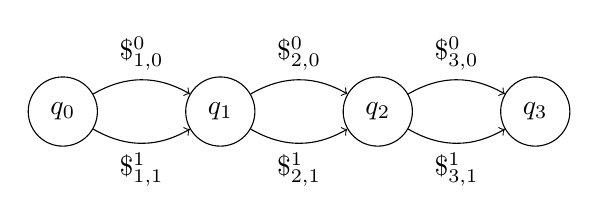
\begin{tikzpicture}[node distance=2cm,on grid,auto]
   \node[state] (q_0)   {$q_0$};
   \node[state] (q_1) [right=of q_0] {$q_1$};
   \node[state] (q_2) [right=of q_1] {$q_2$};
   \node[state] (q_3) [right=of q_2] {$q_3$};
    \path[->]
    (q_0) edge [bend left]  node [above] {$\repl{1}{0}{0}$} (q_1)
          edge [bend right] node [below] {$\repl{1}{1}{1}$} (q_1)
    (q_1) edge [bend left]  node [above] {$\repl{2}{0}{0}$} (q_2)
          edge [bend right] node [below] {$\repl{2}{1}{1}$} (q_2)
    (q_2) edge [bend left]  node [above] {$\repl{3}{0}{0}$} (q_3)
          edge [bend right] node [below] {$\repl{3}{1}{1}$} (q_3);
\end{tikzpicture}
\end{center}

We initially have $x_3 \in L_\vcons$.
We first eliminate $x_3 = y^1_3 \concat z^1_3$ and then
\[
    \begin{array}{rcl}
        y^0_3 &=& \replaceall(x_{1}, \nbit{3}{0}, \repl{3}{0}{0}) \ \land \\
        y^1_3 &=& \replaceall(y^0_3, \nbit{3}{1}, \repl{3}{0}{1}) \ \land \\
        z^0_3 &=& \replaceall(x_{1}, \nbit{3}{0}, \repl{3}{1}{0}) \ \land \\
        z^1_3 &=& \replaceall(z^0_3, \nbit{3}{1}, \repl{3}{1}{1}) \ .
    \end{array}
\]
Note, from $L'_{0}$ we replace the $\repl{3}{0}{0}$- and $\repl{3}{0}{1}$-transitions (although the latter does not appear in $\cA$), while from $L'_{1}$ we replace the $\repl{3}{1}{0}$- and $\repl{3}{1}{1}$-transitions.
This leaves us with
\[
    x_{2} \in L_{0} \land x_{2} \in L_{1}
\]
where $L_{0}$ is given by
\begin{center}
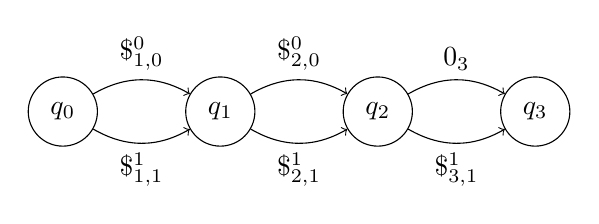
\begin{tikzpicture}[node distance=2cm,on grid,auto]
   \node[state] (q_0)   {$q_0$};
   \node[state] (q_1) [right=of q_0] {$q_1$};
   \node[state] (q_2) [right=of q_1] {$q_2$};
   \node[state] (q_3) [right=of q_2] {$q_3$};
    \path[->]
    (q_0) edge [bend left]  node [above] {$\repl{1}{0}{0}$} (q_1)
          edge [bend right] node [below] {$\repl{1}{1}{1}$} (q_1)
    (q_1) edge [bend left]  node [above] {$\repl{2}{0}{0}$} (q_2)
          edge [bend right] node [below] {$\repl{2}{1}{1}$} (q_2)
    (q_2) edge [bend left]  node [above] {$\nbit{3}{0}$} (q_3)
          edge [bend right] node [below] {$\repl{3}{1}{1}$} (q_3);
\end{tikzpicture}
\end{center}
and $L_{1}$ is given by
\begin{center}
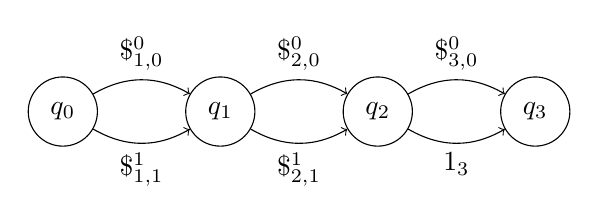
\begin{tikzpicture}[node distance=2cm,on grid,auto]
   \node[state] (q_0)   {$q_0$};
   \node[state] (q_1) [right=of q_0] {$q_1$};
   \node[state] (q_2) [right=of q_1] {$q_2$};
   \node[state] (q_3) [right=of q_2] {$q_3$};
    \path[->]
    (q_0) edge [bend left]  node [above] {$\repl{1}{0}{0}$} (q_1)
          edge [bend right] node [below] {$\repl{1}{1}{1}$} (q_1)
    (q_1) edge [bend left]  node [above] {$\repl{2}{0}{0}$} (q_2)
          edge [bend right] node [below] {$\repl{2}{1}{1}$} (q_2)
    (q_2) edge [bend left]  node [above] {$\repl{3}{0}{0}$} (q_3)
          edge [bend right] node [below] {$\nbit{3}{1}$} (q_3);
\end{tikzpicture}
\end{center}


After completing the elimination process, we are left with
\[
    x_1 \in L_{000} \land \ldots \land x_1 \in L_{111}
\]
where, for example, $L_{010}$ is given by
\begin{center}
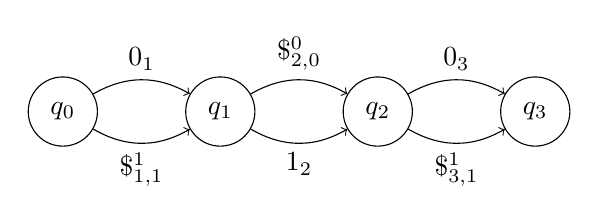
\begin{tikzpicture}[node distance=2cm,on grid,auto]
   \node[state] (q_0)   {$q_0$};
   \node[state] (q_1) [right=of q_0] {$q_1$};
   \node[state] (q_2) [right=of q_1] {$q_2$};
   \node[state] (q_3) [right=of q_2] {$q_3$};
    \path[->]
    (q_0) edge [bend left]  node [above] {$\nbit{1}{0}$} (q_1)
          edge [bend right] node [below] {$\repl{1}{1}{1}$} (q_1)
    (q_1) edge [bend left]  node [above] {$\repl{2}{0}{0}$} (q_2)
          edge [bend right] node [below] {$\nbit{2}{1}$} (q_2)
    (q_2) edge [bend left]  node [above] {$\nbit{3}{0}$} (q_3)
          edge [bend right] node [below] {$\repl{3}{1}{1}$} (q_3);
\end{tikzpicture}
\end{center}
If we further insist that $x_1$ contains only characters from
$\set{\nbit{1}{0},
      \nbit{1}{1},
      \nbit{2}{1},
      \nbit{2}{1},
      \nbit{3}{1},
      \nbit{3}{1}}$
then the only path from $q_0$ to $q_3$ is via the sequence
$\nbit{1}{0} \nbit{2}{1} \nbit{3}{0}$.
Likewise, in $L_{111}$ the only valid sequence will be
$\nbit{1}{1} \nbit{2}{1} \nbit{3}{1}$.


\subsection{Completing the Reduction}

To finish the reduction, we have to instantiate $\varphi$ by giving
$L$, $L_\hcons$, $L_1$, \ldots, $L_n$ and $L_\vcons$ where all languages but $L_\vcons$ are easily seen to be representable by automata whose size is polynomial in $n$.
\begin{enumerate}
\item
    $L$ will enforce that $x_1$ matches
    \[
        \resetchar
        \brac{
            \rowdelim
            \brac{
                \set{\nbit{1}{0},\nbit{1}{1}}
                \cdots
                \set{\nbit{n}{0},\nbit{n}{1}}
                \tiles
            }^\ast
        }^\ast
        \rowdelim
        \resetchar \ .
    \]
    That is, a sequence of delimited rows, each consisting of a sequence of alternating $n$-bit sequences and tiles;
    the beginning and end of the word is marked by $\resetchar$.
    Moreover, $L$ will insist that the first tile seen is $\inittile$ and that the final tile seen is $\fintile$, as required by the tiling problem.

\item
    $L_\hcons$ will enforce that any subsequence
    \[
        \tile \bit_1 \ldots \bit_n \tile'
    \]
    where for all $i$ we have
    $\bit_i \in \set{\nbit{i}{0}, \nbit{i}{1}}$
    in the value of $x_1$ is such that $\tup{\tile, \tile'} \in \hcons$.

\item
    The languages $L_1, \ldots L_n$ will together enforce the correct sequencing of bit values $\bit_1 \ldots \bit_n$.
    That is, between each $\rowdelim$ each sequence $\bit_1 \ldots \bit_n$ appears exactly once and in the correct order
    (i.e.\ %
    $\nbit{1}{0}\ldots\nbit{n-1}{0}\nbit{n}{0}$
    appears before
    $\nbit{1}{0}\ldots\nbit{n-1}{0}\nbit{n}{1}$
    and so on up to
    $\nbit{1}{1}\ldots\nbit{n-1}{1}\nbit{n}{1}$).
    To do this, each $L_i$ will check the following.
    \begin{enumerate}
    \item
        After each $\rowdelim$ the first instance of
        $\set{\nbit{i}{0},\nbit{i}{1}}$
        is $\nbit{i}{0}$.
    \item
        Before each $\rowdelim$ the last instance of
        $\set{\nbit{i}{0},\nbit{i}{1}}$
        is $\nbit{i}{1}$.
    \item
        For every $\nbit{i}{0}$ such that
        $\rowdelim$ does not appear before the next occurrence of
        $\bit_i \in \set{\nbit{i}{0},\nbit{i}{1}}$,
        if the immediately succeeding characters are
        $\nbit{i+1}{1}\ldots\nbit{n}{1}$
        then $\bit_i$ is $\nbit{i}{1}$,
        otherwise $\bit_i$ is $\nbit{i}{0}$.
    \item
        For every $\nbit{i}{1}$ such that
        $\rowdelim$ does not appear before the next occurrence of
        $\bit_i \in \set{\nbit{i}{0},\nbit{i}{1}}$,
        if the immediately succeeding characters are
        $\nbit{i+1}{1}\ldots\nbit{n}{1}$
        then $\bit_i$ is $\nbit{i}{0}$,
        otherwise $\bit_i$ is $\nbit{i}{1}$.
    \end{enumerate}
    \mat{I think i've got this right: it's standard if not...}
\end{enumerate}

Finally, we need to define $L_\vcons$.
As seen above, $L_\vcons$ will lead to an exponential number of languages
$L_{\bit_1\ldots\bit_n}$
inside which $x_1$ will need to be contained.
The role of
$L_{\bit_1\ldots\bit_n}$
will be to check that the
$\bit_1\ldots\bit_n$th
column of the tiling obeys the vertical matching relation.
Each
$L_{\bit_1\ldots\bit_n}$
can be seen to be representable by a polynomially sized automaton that stores in its states the last tile seen after the sequence
$\bit_1\ldots\bit_n$.
Then, when the sequence next occurs, the new tile can be compared with the previous one.
The automaton will proceed by storing the new tile and forgetting the old.

We will design an automaton for $L_\vcons$ which will lead to the generation of the correct automaton for each
$L_{\bit_1\ldots\bit_n}$.
We will use characters
$\repl{i}{\bit}{\bit'}$
as before to generate the required bit sequences in the transition labelling of the automaton representing
$L_{\bit_1\ldots\bit_n}$.

In addition, we also need to ensure that the elimination of the concatenations -- which leads to a non-deterministic change in the initial and final states of the automata -- does not disrupt the language accepted.
For this we will use the $\resetchar$ character, which marks the beginning and end of the value of $x_1$.
The automaton for $L_\vcons$ will treat $\resetchar$ as a kind of ``reset'' character, which takes the automaton back to a defined initial state, which will also be the accepting state.

Before giving the formal definition, we will give an extract of the automaton that will check for the sequence
$\bit_1\ldots\bit_n$
and check the tiling relation.
Each state is of the form $\tup{q, \tile}$ where $\tile$ is the previously saved tile.
In the diagram, $\replall{i}$ denotes the set of all characters
$\repl{i}{\bit}{\bit'}$
for all $\bit, \bit' \in \set{0,1}$.
I.e.\ the transition can read any of these characters.
The top row of the automaton shows the run whilst the correct sequence is being read (and the tile needs to be checked), whilst the bottom is for all bit sequences that diverge from
$\bit_1\ldots\bit_n$
(another column is being read).
From $\tup{q_n, \tile}$ the tiles
$t_1, \ldots, t_m$
are all tiles such that
$\tup{t, t_j} \in \vcons$
for all $j$.
The transitions from each
$\tup{q_1, \tile_j}$
will be analogous to those from
$\tup{q_1, \tile}$.

\scalebox{.8}{
    \begin{center}
    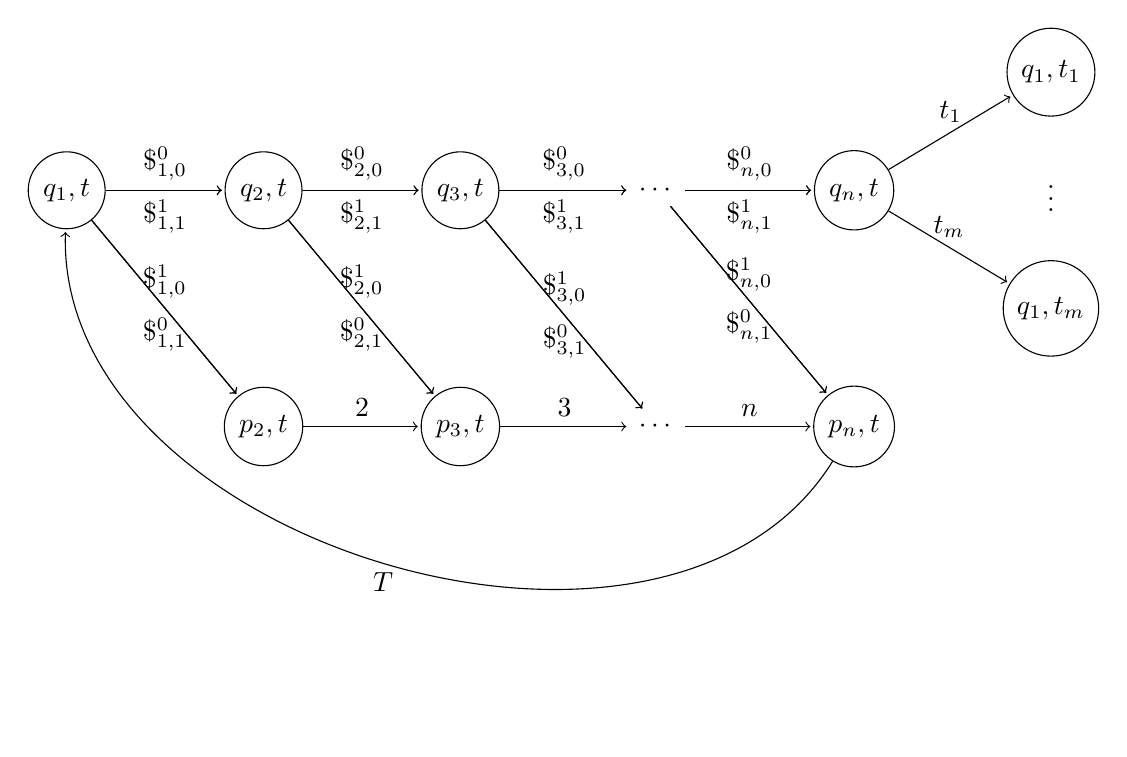
\begin{tikzpicture}[node distance=3cm and 2.5cm,on grid,auto,bend angle=75,shorten >= 1pt]
       \node[state] (q1)   {$\tup{q_1, \tile}$};
       \node[state] (q2) [right=of q1] {$\tup{q_2, \tile}$};
       \node[state] (q3) [right=of q2] {$\tup{q_3, \tile}$};
       \node        (qdots) [right=of q3] {$\cdots$};
       \node[state] (qn) [right=of qdots] {$\tup{q_n, \tile}$};
       \node[state] (qt1) [above right=of qn,yshift=-1.5cm] {$\tup{q_1, \tile_1}$};
       \node        (qtdots) [right=of qn] {$\vdots$};
       \node[state] (qtm) [below right=of qn,yshift=1.5cm] {$\tup{q_1, \tile_m}$};
       \node[state] (p2) [below=of q2] {$\tup{p_2, \tile}$};
       \node[state] (p3) [below=of q3] {$\tup{p_3, \tile}$};
       \node        (pdots) [below=of qdots] {$\cdots$};
       \node[state] (pn) [below=of qn] {$\tup{p_n, \tile}$};
       \path[->]
         (q1) edge node [above] {$\repl{1}{0}{0}$} (q2)
         (q1) edge node [below] {$\repl{1}{1}{1}$} (q2)
         (q1) edge node [above] {$\repl{1}{0}{1}$} (p2)
         (q1) edge node [below] {$\repl{1}{1}{0}$} (p2)
         %
         (q2) edge node [above] {$\repl{2}{0}{0}$} (q3)
         (q2) edge node [below] {$\repl{2}{1}{1}$} (q3)
         (q2) edge node [above] {$\repl{2}{0}{1}$} (p3)
         (q2) edge node [below] {$\repl{2}{1}{0}$} (p3)
         %
         (q3) edge node [above] {$\repl{3}{0}{0}$} (qdots)
         (q3) edge node [below] {$\repl{3}{1}{1}$} (qdots)
         (q3) edge node [above] {$\repl{3}{0}{1}$} (pdots)
         (q3) edge node [below] {$\repl{3}{1}{0}$} (pdots)
         %
         (qdots) edge node [above] {$\repl{n}{0}{0}$} (qn)
         (qdots) edge node [below] {$\repl{n}{1}{1}$} (qn)
         (qdots) edge node [above] {$\repl{n}{0}{1}$} (pn)
         (qdots) edge node [below] {$\repl{n}{1}{0}$} (pn)
         %
         (p2) edge node [above] {$\replall{2}$} (p3)
         (p3) edge node [above] {$\replall{3}$} (pdots)
         (pdots) edge node [above] {$\replall{n}$} (pn)
         %
         (pn) edge [bend left] node [below] {$\tiles$} (q1)
         (qn) edge node [above] {$\tile_1$} (qt1)
         (qn) edge node [above] {$\tile_m$} (qtm);
    \end{tikzpicture}
    \end{center}
}

To see the pattern of the automaton extract, we show how it would be instantiated for $L_{0\ldots00}$ with all edges labelled by
$\repl{i}{\bit}{\bit'}$
removed.

\scalebox{.8}{
    \begin{center}
    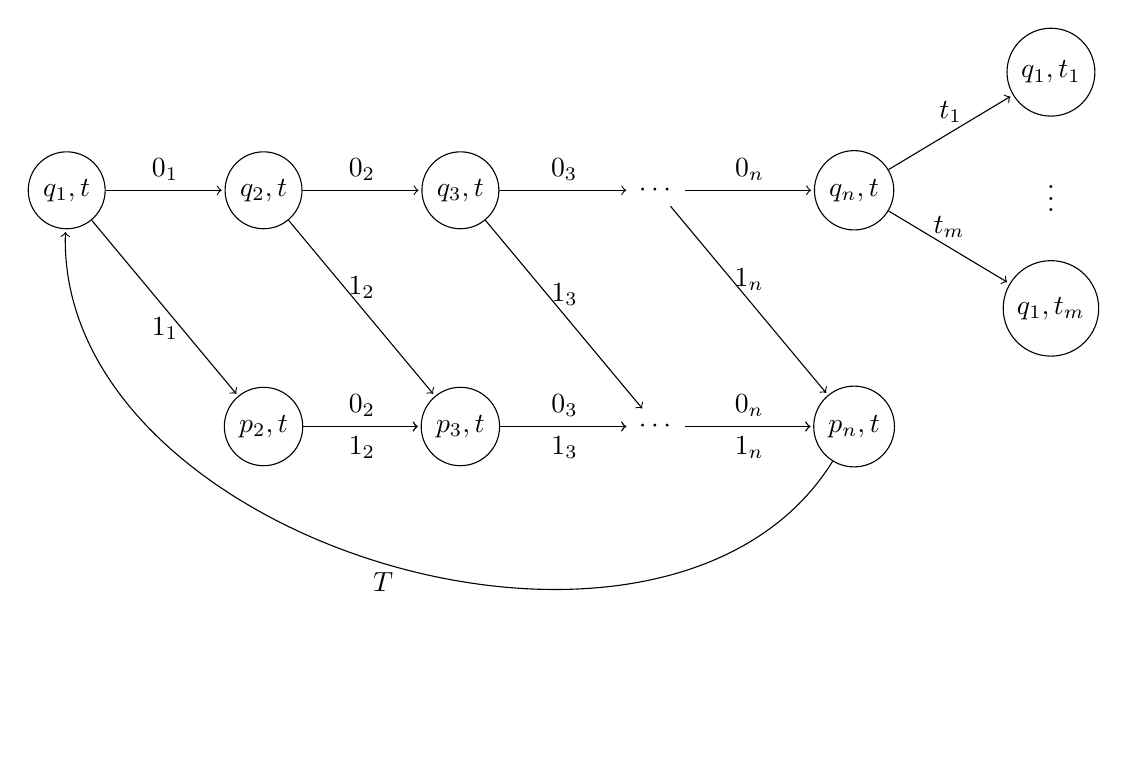
\begin{tikzpicture}[node distance=3cm and 2.5cm,on grid,auto,bend angle=75,shorten >= 1pt]
       \node[state] (q1)   {$\tup{q_1, \tile}$};
       \node[state] (q2) [right=of q1] {$\tup{q_2, \tile}$};
       \node[state] (q3) [right=of q2] {$\tup{q_3, \tile}$};
       \node        (qdots) [right=of q3] {$\cdots$};
       \node[state] (qn) [right=of qdots] {$\tup{q_n, \tile}$};
       \node[state] (qt1) [above right=of qn,yshift=-1.5cm] {$\tup{q_1, \tile_1}$};
       \node        (qtdots) [right=of qn] {$\vdots$};
       \node[state] (qtm) [below right=of qn,yshift=1.5cm] {$\tup{q_1, \tile_m}$};
       \node[state] (p2) [below=of q2] {$\tup{p_2, \tile}$};
       \node[state] (p3) [below=of q3] {$\tup{p_3, \tile}$};
       \node        (pdots) [below=of qdots] {$\cdots$};
       \node[state] (pn) [below=of qn] {$\tup{p_n, \tile}$};
       \path[->]
         (q1) edge node [above] {$\nbit{1}{0}$} (q2)
         (q1) edge node [below] {$\nbit{1}{1}$} (p2)
         %
         (q2) edge node [above] {$\nbit{2}{0}$} (q3)
         (q2) edge node [above] {$\nbit{2}{1}$} (p3)
         %
         (q3) edge node [above] {$\nbit{3}{0}$} (qdots)
         (q3) edge node [above] {$\nbit{3}{1}$} (pdots)
         %
         (qdots) edge node [above] {$\nbit{n}{0}$} (qn)
         (qdots) edge node [above] {$\nbit{n}{1}$} (pn)
         %
         (p2) edge node [above] {$\nbit{2}{0}$} (p3)
         (p2) edge node [below] {$\nbit{2}{1}$} (p3)
         (p3) edge node [above] {$\nbit{3}{0}$} (pdots)
         (p3) edge node [below] {$\nbit{3}{1}$} (pdots)
         (pdots) edge node [above] {$\nbit{n}{0}$} (pn)
         (pdots) edge node [below] {$\nbit{n}{1}$} (pn)
         %
         (pn) edge [bend left] node [below] {$\tiles$} (q1)
         (qn) edge node [above] {$\tile_1$} (qt1)
         (qn) edge node [above] {$\tile_m$} (qtm);
    \end{tikzpicture}
    \end{center}
}

Hence, we are ready to define an automaton $\cA_\vcons$ giving the language $L_\vcons$.
We give the definition first, and explanation below.
We define
\[
    \cA_\vcons = \tup{Q, \delta, q_0, F}
\]
where
\[
    \begin{array}{rcl}
        Q &=& \set{q_0, \ldots, q_n, p_2, \ldots, p_n} \ \cup \\
          & & \setcomp{\tup{q_i, \tile}}
                      {0 \leq i \leq n \land \tile \in \tiles} \ \cup \\
          & & \setcomp{\tup{p_i, \tile}}
                      {2 \leq i \leq n \land \tile \in \tiles} \\
        \\
        \delta &=& \setcomp{q \xrightarrow{\resetchar} q_0}{q \in Q} \ \cup \\
               & & \set{q_0 \xrightarrow{\rowdelim} q_1} \cup
                   \setcomp{\tup{q_0, \tile}
                            \xrightarrow{\rowdelim}
                            \tup{q_1, \tile}}
                           {\tile \in \tiles} \ \cup \\
               & & \setcomp{q_i
                            \xrightarrow{\repl{i}{\bit}{\bit}}
                            q_{i+1}}
                           {1 \leq i < n \land \bit \in \set{0,1}} \ \cup \\
               & & \setcomp{\tup{q_i, \tile}
                            \xrightarrow{\repl{i}{\bit}{\bit}}
                            \tup{q_{i+1}, \tile}}
                           {1 \leq i < n \land \bit \in \set{0,1}} \ \cup \\
               & & \setcomp{q_i
                            \xrightarrow{\repl{i}{\bit}{\bit'}}
                            p_{i+1}}
                           {1 \leq i < n \land
                            \bit \neq \bit' \in \set{0,1}} \ \cup \\
               & & \setcomp{\tup{q_i, \tile}
                            \xrightarrow{\repl{i}{\bit}{\bit'}}
                            \tup{p_{i+1}, \tile}}
                           {1 \leq i < n \land
                            \bit \neq \bit' \in \set{0,1}} \ \cup \\
               & & \setcomp{p_i
                            \xrightarrow{\repl{i}{\bit}{\bit'}}
                            p_{i+1}}
                           {2 \leq i < n \land \bit, \bit' \in \set{0,1}} \ \cup \\
               & & \setcomp{q_n \xrightarrow{\tile} \tup{q_0, \tile}}
                           {\tile \in \tiles} \ \cup \\
               & & \setcomp{\tup{q_n, \tile}
                            \xrightarrow{\tile'}
                            \tup{q_0, \tile'}}
                           {\tup{\tile, \tile'} \in \vcons} \ \cup \\
               & & \setcomp{\tup{p_n, \tile}
                            \xrightarrow{\tile'}
                            \tup{q_0, \tile'}}
                           {\tile, \tile' \in \tiles} \\
        \\
        F &=& \set{q_0}
    \end{array}
\]
The first set of transitions in $\delta$ are the reset transitions.
From all states (including $q_0$) a $\resetchar$ will bring the automaton back to its initial state.
Since we enforce separately that the value of $x_0$ begins and ends with $\resetchar$, it will remain true through the concatenations and $\replaceall$ operations that the value of $x_i$ still begins and ends with $\resetchar$.
Thus, the only final state that can occur on a solution to the string constraints is $q_0$ and the initial state is immaterial.

Next, we define the transitions over $\rowdelim$ which simply track the beginning of a new row.

The next transitions read
$\repl{i}{\bit}{\bit}$
characters.
This means that in
$L_{\bit_1 \ldots \bit_n}$
we are reading the value $\bit = \bit_i$ at position $i$.
Thus, this is part of the sequence of bits identifying the column
$L_{\bit_1 \ldots \bit_n}$
is checking.
\mat{Is this confusing?}
Thus, we continue reading the sequence of bits in the $q$ states.

Conversely, we next deal with the case when
$\repl{i}{\bit}{\bit'}$
with $\bit \neq \bit'$ is being read.
That is, we are reading a column that is not the
$\bit_1\ldots\bit_n$th
and hence we simply skip over it by using the $p$ states.

Finally, we read the tiles.
If we are in state $q_n$ then we are reading the
$\bit_1\ldots\bit_n$th
column, but this is the first row (after a reset) and thus there is no matching relation to verify.
If we are in state $\tup{q_n, \tile}$ then we are reading the
$\bit_1\ldots\bit_n$th
column, but this is the not the first row and we have to verify the matching relation.
Wherefrom, there is only a transition reading $\tile'$ if
$\tup{\tile, \tile'} \in \vcons$.
The tile $\tile'$ is then saved for comparison with the next tile.

Otherwise, if we are in a state $p_n$ or $\tup{p_n, \tile}$ then we are not in the correct column and there is nothing to verify.
In this case we simply skip over the tile and continue.


\subsection{Conclusion}

Given a tiling problem over a corridor of width $2^n$, we have given a (polynomially sized in $n$)
$\strline[\replaceall]$
constraint $\varphi$ using languages
$L$, $L_\vcons$, $L_\hcons$, $L_1$, \ldots, $L_n$
(representable by automata polynomially sized in $n$)
such that $\varphi$ is satisfiable iff the variable $x_1$ takes on a value
\[
    \resetchar
    \rowdelim \nbit{1}{0} \cdots \nbit{n}{0} \tile^1_1
              \nbit{1}{0} \cdots \nbit{n}{1} \tile^1_2
              \cdots
              \nbit{1}{1} \cdots \nbit{n}{1} \tile^1_\width
    \rowdelim \cdots
    \rowdelim \nbit{1}{0} \cdots \nbit{n}{0} \tile^\height_1
              \cdots
              \nbit{1}{1} \cdots \nbit{n}{1} \tile^\height_\width
    \rowdelim
    \resetchar
\]
such that
\[
    \rowdelim \tile^1_1 \cdots \tile^1_\width
    \rowdelim \tile^2_1 \cdots \tile^2_\width
    \rowdelim \cdots
    \rowdelim \tile^\height_1 \cdots \tile^\height_\width
    \rowdelim
\]
is a solution to the tiling problem.
Since such a tiling problem is $2^n$-SPACE-hard, we have shown EXPSPACE-hardness of
the satisfiability problem for $\strline[\replaceall]$, moreover, this holds even in the single-letter case.
\mat{
    The previous pages are a proof of this, i think.
    Let me know if you would like something more formal.
}


\end{document}
